\documentclass[a4paper,11pt,twocolumn]{jsarticle}
\usepackage{here}
\usepackage[dvipdfmx,nosetpagesize]{graphicx,color}
\usepackage[T1]{fontenc}
\usepackage{url}
\usepackage{subcaption}
\usepackage{indentfirst}
\usepackage{comment}
\usepackage{here}
\usepackage{stfloats} 
\usepackage{graphicx}
\graphicspath{ {./images/} }

\usepackage{array}  % for multilne tabular
\newcolumntype{M}[1]{>{\centering\arraybackslash}m{#1}}

%%% spacing
\usepackage{setspace}
\setstretch{0.8}

\usepackage{geometry}
\geometry{left=10truemm,right=10truemm,top=13truemm,bottom=28truemm}
\renewcommand{\refname}{参考リスト}%参考文献の文字を消す
%

\usepackage{titlesec}
\titleformat*{\section}{\Large\bfseries}
\titlespacing*{\section}{1truemm}{2truemm}{2truemm}
\titlespacing*{\subsection}{0pt}{3truemm}{0pt}

% \setlength\intextsep{2mm}
% \setlength\textfloatsep{2mm}

% 図と図の間のスペース
\setlength\floatsep{0truemm}
% 本文と図の間のスペース
% 本文中の図のスペース
% \setlength\intextsep{0pt}
% 図とキャプションの間のスペース
\setlength\abovecaptionskip{0truemm}

% 段抜きの上下?マージン
\setlength\dbltextfloatsep{0truemm}

%%% alias

\newcommand{\figref}[1]{{図~\ref{#1}}}
\newcommand{\tabref}[1]{{表~\ref{#1}}}

\RequirePackage[l2tabu, orthodox]{nag}

\begin{document}
\twocolumn[
{
  \hrulefill
  \begin{center}
  {\number2025 年\number5 月\number23 日}HPC講座 研究室内発表会

  \smallskip
  \Large{スーパーコンピュータ「富岳」における故障ノードに関する研究}
  
  \medskip
  \begin{tabular}{rc}
    発表者:& 坂上創哉\\
    所属:& 三輪研究室\\
    指導教員:& 三輪 忍 准教授 \\
  \end{tabular}
  \end{center}
  \smallskip
  \hrulefill
  \bigskip
  }]

\section{はじめに}
スーパーコンピュータの運用では,大量の計算ノードを扱うため,月に数十件の障害が発生することが報告されている\cite{HPC_system_fail}.計算ノードはマザーボードに固定されており,一つの計算ノードが故障した場合でも,CMU単位での交換が必要となる.このような障害は運用コストの増加やユーザーの利便性の低下を招くため,可能な限り減少させる必要がある.本研究では,「富岳」における故障ノードのログを分析し,故障の傾向や相関関係を明らかにすることを目的とする.


\section{研究背景}

\subsection{スーパーコンピュータ「富岳」}\label{sec:fugaku}
「富岳」は,理化学研究所と富士通が共同開発した日本を代表するスーパーコンピュータである.2020年6月に稼働を開始し,2020年11月にはTOP500ランキングで世界1位を獲得した\cite{HPCG}.「富岳」は,ARMアーキテクチャを採用したA64FXプロセッサと,最大で158,976ノードの計算ノードを持つ\cite{Fugaku_Web}.また,計算タスクのみを実行するノードは,アクティブ光ケーブル(AOC)ノードとnon-AOCノードの2種類に分けられる.AOCノードはアクティブ光ケーブルに電力を供給し,non-AOCノードは電力を供給しない
富岳は,一般的な汎用ソフトで動き,シミュレーションやビッグデータ,AIなど幅広いアプリケーションで高性能を発揮するように設計されている.

\subsection{ノードの故障}
富岳の試行運用開始である2020年4月1日から2024年10月31日までの期間に記録されたCMUの障害ログは,全1,873件であり,このうち,CPUまで特定されている障害件数は1,579件であると報告されている.\cite{master_kusaba}.また,富岳以前に理化学研究所で運用されていたスーパーコンピュータ「京」では,2012年9月28日から2015年6月30日までの稼働をしていた.月別のCPUの故障率は高負荷時を除いて0.004\%程度で概ね安定している\cite{k_HPC}図\ref{fig:Kfail}.0.004\%とは毎月3.3件の故障であり,9日に1個程度である.

\begin{figure}[h]
  \centering
  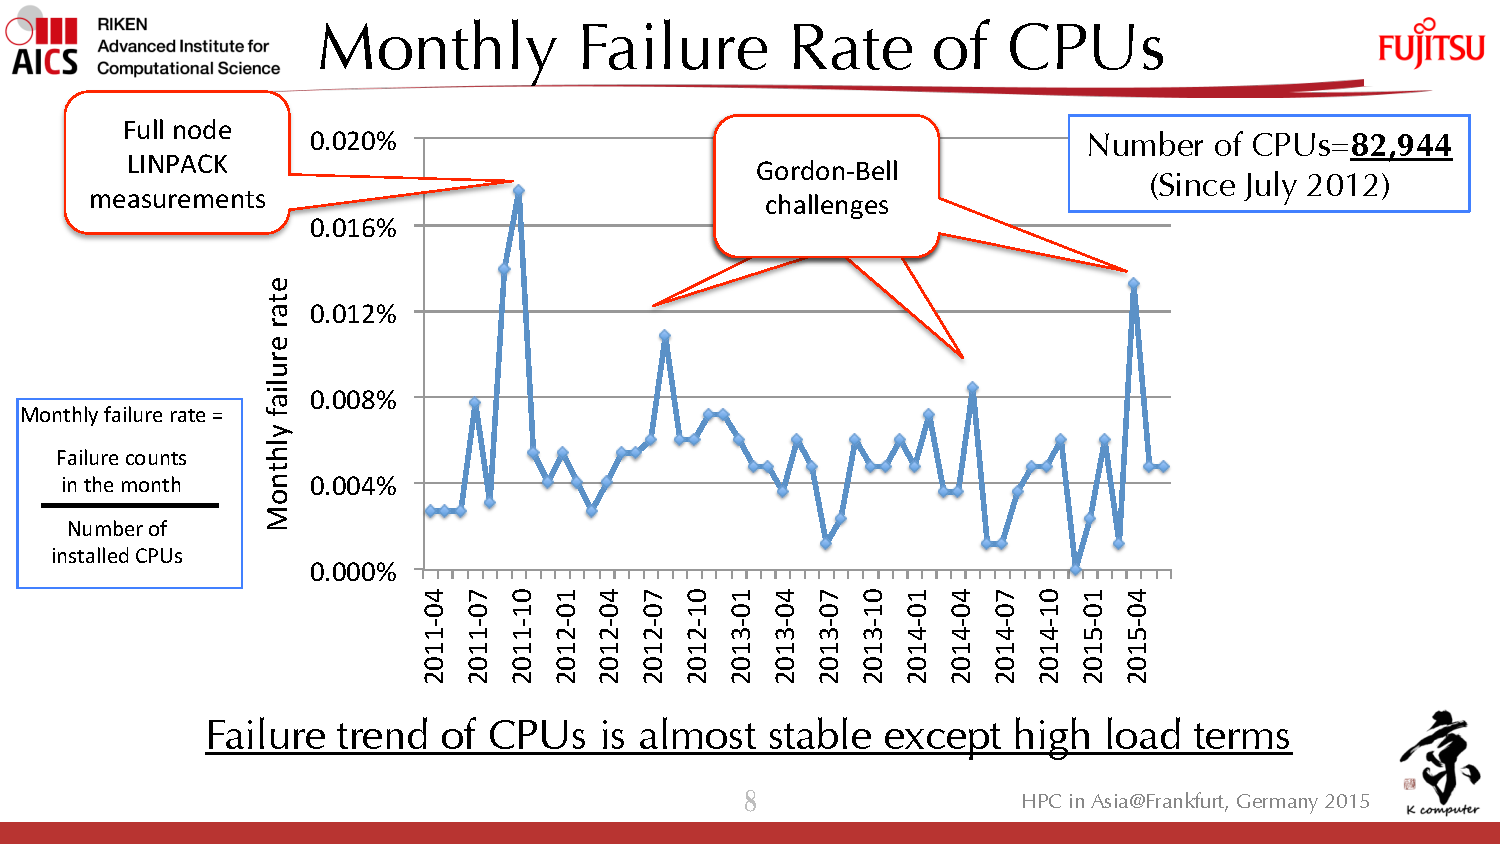
\includegraphics[width=0.8\linewidth]{figure/Kfail.pdf}
  \caption{「京」の月別CPU故障率(文献\cite{k_HPC})より}
  \label{fig:Kfail}
\end{figure}

\subsection{電力ばらつきと故障}
一般的なスーパーコンピュータは,同一仕様の計算ノードがネットワークを介して接続されているため,これらの計算ノードは,与えられたアプリケーションに対して同一の消費電力を示すことが期待されている.しかし,実際には半導体チップの製造上のばらつきが存在するため,同一のアプリケーションを実行してもそれぞれ異なる消費電力を示すことが報告されている.文献\cite{master_kusaba}では,CPUの故障要因の一つとして,温度を挙げている.CPUの温度は消費電力に依存しており,消費電力が高いほどCPUの温度も上昇するため,消費電力のばらつきがCPUの故障に影響を与えると考えられる.文献\cite{master_kusaba}では,消費電力と故障率の相関関係を調査した結果,消費電力のばらつきと故障率の間に明確な関係性はみられなかったと報告されている.
図\ref{fig:Fugakufail}は富岳における消費電力と故障ノードの分布を示しており,ひし形で強調された点が故障したノードを表している.故障ノードは,消費電力に関わらず,分布していることが確認できる.また,表\ref{tab:power}は,富岳のnon-AOCノードにおける消費電力を示している.全体の平均消費電力は142.1Wであり,故障ノードの平均消費電力は141.8Wである.故障ノードの平均消費電力は全体の平均消費電力とほぼ同じであり,故障ノードの消費電力は全体の平均消費電力とほぼ同じであることがわかる.

\begin{table}[h]
  \centering
  \caption{non-AOCノードにおける消費電力(文献\cite{master_kusaba})より}
  \label{tab:power}
  \begin{tabular}{c|cc}
    \hline
    種類 & 数量 & 平均消費電力(W) \\
    \hline 
    \hline
    全non-AOCノード & 12,672 & 142.1  \\
    全故障ノード & 107 & 141.8  \\
    \hline
    要因:CPU & 37 & 141.9 \\
    要因:メモリ & 70 & 141.8 \\
    \hline
  \end{tabular}
\end{table}

\begin{figure}[h]
  \centering
  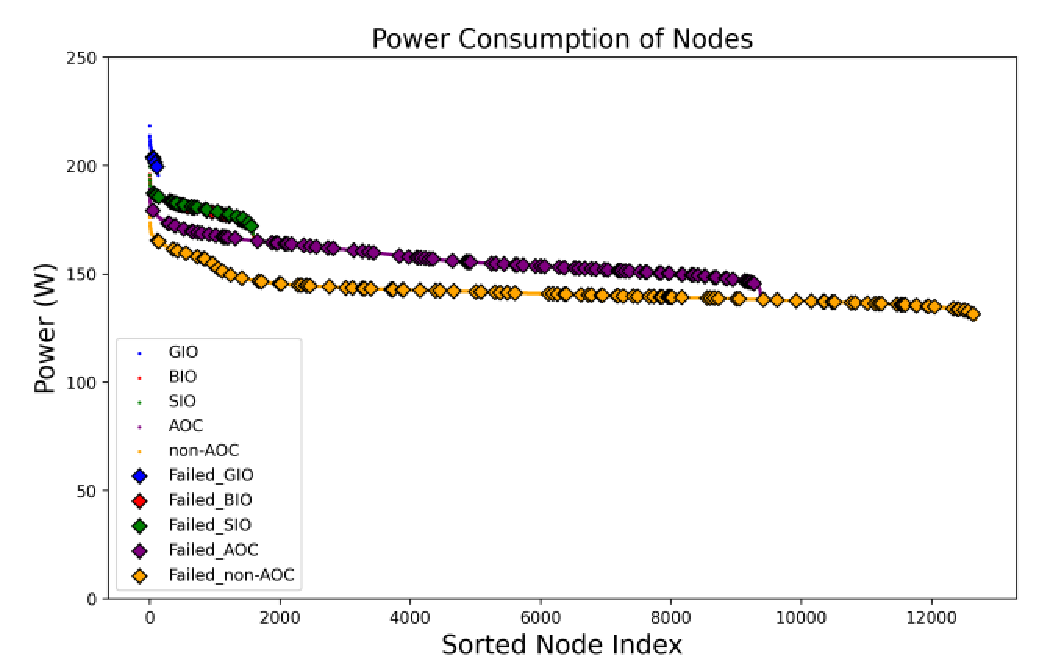
\includegraphics[width=8cm]{figure/Fugakufail.pdf}
  \caption{富岳における消費電力と故障ノードの分布(文献\cite{master_kusaba})より}
  \label{fig:Fugakufail}
\end{figure}

\section{先行研究}
文献\cite{HPC_system_fail}では,ロスアラモス研究所が10年間に渡り収集したデータを用いて,HPCシステムにおける故障の予測因子やその関連性を詳しく分析している.HPCシステムにおける故障の傾向を広範に調査し,時間的・空間的な相関,故障原因の性質,およびノードの使用状況や環境要因が,故障の発生に大きな影響を与えることを明らかにしている.また,文献\cite{master_kusaba}では,富岳における電力ばらつきがノード故障率に与える影響を調査している.富岳の電力ばらつきと故障の関係について,故障ノードの平均消費電力とノード全体の平均消費電力の差はわずか0.3Wであり,消費電力の差はほとんど見られず,電力ばらつきと故障率の関係性はあまり見られなかったと報告された.

\section{研究目的}
本研究では,電力ばらつきと故障の関係性が見られなかったことから,ノードの故障率には,使用率や実行されるジョブの種類が影響を与える可能性があると考えられる.
富岳の故障ノードのログを詳細に分析し,故障の傾向や相関関係を明らかにすることを目的とする.


\section{今後の予定}

\begin{itemize}
  \item 富岳の故障ノードのログを分析し,故障の傾向や相関関係を明らかにする.
  \item 故障ノードのログを基に,故障の予測モデルを構築する.
  \item 故障の予測モデルを用いて,富岳の運用における故障率を低下させるための提案を行う.
\end{itemize}

\bibliography{references}
\bibliographystyle{ipsjsortEX}


\end{document}

